\chapter{Project Management}
\label{project management}

\section{The Group}
The group formed out of the desire to work together based on varying levels of previous experience working together, rather than out of a desire to work on a specific project as was the case with other groups.
The group quickly decided to take advantage of the new iLab at Warwick University \cite{Kalvala2013} and chose to make use of the Microsoft Kinect. Initial ideas revolved around object modelling and sharing, but due to the low resolution and minimum scanning distance of the Kinect, these early ideas were abandoned. It is from these ideas that the name ``PARSE" was created as this was an acronym for an early project title. After discussions with the project supervisor, the group chose to tackle the problem proposed by Dr. Paul Summers of the European Institute of Oncology and Prof. Massimo Pelligrini of the Clinical and Public Health University of Italy. \\

This section provides a comprehensive description of the project management techniques and group organisation used by the team during the course of this project. \\

\section{Team Members and Roles}

\begin{figure}[h]
    \begin{center}
        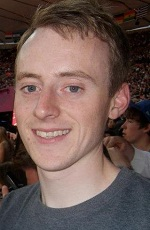
\includegraphics[scale=0.5]{images/bernard}
        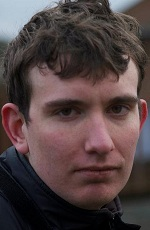
\includegraphics[scale=0.5]{images/greg}
        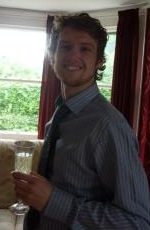
\includegraphics[scale=0.5]{images/nathan}
        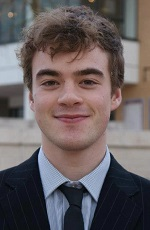
\includegraphics[scale=0.5]{images/robin}
        
\includegraphics[scale=0.5]{images/stef} 
        \end{center}
        \caption{The group from left to right: Bernard, Greg, Nathan, Robin and Stefania.}
    \label{fig:the group}
\end{figure}

The main focus of the initial meetings at the start of the project was to identify each member’s core competencies and to allow the members to become familiar and comfortable with one another. This process created a productive and friendly yet professional atmosphere which set the grounds for the smooth development of the project. All members of the group had a great deal of experience with Java, therefore C\# was chosen as the programming language due to the numerous syntactic similarities. \\

Individuals were responsible for the research, design, implementation and testing of specific areas. Bernard was responsibly for UI design, database connectivity and leading the project. Greg was responsible for person isolation and volume estimation. Nathan was responsible for scanner recognition. Robin was responsible for ensuring the shared work space was maintained, data structures and point cloud registration. Stefania was responsible for the skeleton tracking, sensor recognition and database connectivity. \\

\section{Group Behaviour}
This section details the working practises and methodologies adopted by the group. \\

\subsection{Weekly Meetings}
In order for this relatively large scale project to be successfully managed alongside the many tasks, activities and commitments which also had to be carried out by the group members as part of their university work, efficient communication was crucial. The group quickly took to organising weekly meeting. In these meetings, which were generally an hour long, the progress of the previous weeks activities could be ascertained and if necessary, more resources added to a outstanding task to ensure it's timely completion. If the previous weeks tasks had been completed, a new task for the upcoming week would be assigned to group members during this time. \\

As a result of the weekly meetings, each group member was assigned a task weekly and as such each member had a clear responsibility for their given task. \\

Additionally, the group would often congregate around the Kinect in CS0.01 within the Computer Science Department at Warwick to work on the project. The group would use these occasions to provide fresh insight into individual problems and was often the setting for the peer review process. \\

\subsection{Communicating with the Supervisor and Client}
Less frequent meetings were also organised between the group and the project supervisor and client in order to provide the latter with a comprehensive update of the project's status. \\

\subsection{Group Methodologies}
At the start, the group timetabled tasks in a strict and regimented way using a Gannt chart, contained in the specification document. From this, the group could agree that at any given point in the time frame we would be working on a particular phase of the project. However, this timetable was very high level and only ever treated as a guide. In practice, our development methodology, especially the implementation phase, was close in style to the agile development family. Our weekly meetings would highlight tasks in the upcoming week that needed to be completed and the group would sub divide into self-organising, cross-functional teams in order to complete those tasks. Hence the group adopted an adaptive approach to planning. Based on the adaptive planning and the fact the group “time-boxed” its iterations into weekly segments, the agile approach could be described as a “Scrum”. \\

%an image of git shit

Often, once tasks had been allocated, based on the the guiding timetable and weekly meeting, the group would subdivide into sub committees and work on tasks together. This division meant that a subset of the group could focus on one particular problem in isolation. In addition, the group would informally demo the latest work to the group.These demos gave the opportunity for the group to feedback and comment on any assumptions that had been made to get the section working, such as the volume estimator assuming the person is an amorphous blob. The group made use of a Git repository \cite{githole} to manage source code, which whilst it had a steep learning curve, has avoided any version control issues. \\

\subsection{Project Timetable and Progress Review}

Our progress when aligned against our project timetable determined at the start of the project went largely to plan. We were able to establish the requirements of the project fairly early on after the idea was conceived. Our research, prototype and develop methodology allowed us to build on ideas found in research immediately and incorporate them into the project if said prototyping produced sufficient and successful results. One area however that did overrun was the technical implementation of the project which took away time from vital testing and calibration of the volume calculation and limb circumference efforts. It also gave us less time to reflect on our results and assure greater accuracy when it came to producing the final report deliverable. This was due to the issues experienced at the start of the project where particular language choices and available frameworks for automating some of the cloud processing in prototyping provided fruitless and unsuitable for the toolkit itself. Regardless of this progress setback, we were able to complete the remainder of the tasks in parallel and satisfy all deliverables appropriately. The project timetable is included as part of the Specification in Appendix A.

\subsection{Final Report}
The writing of this final report, fortunately, was started early in second term, which allowed us not only to make swift progress, but to iron out some serious issues. Storing and working on the document source in our Git repository soon proved to be problematic, with almost all changes resulting in file-wide conflicts. Left unchanged, this situation would seriously impede our efforts for the coming months.\\

The solution was to use a dedicated service to store, manage and edit the LaTeX project, and after significant research into this yet-developing service, we settled with the ShareLaTeX service \cite{sharedurex}. Their efforts and highly personable service enabled us to collaborate swiftly and without further major issues. \\

